
\chapter{Feynman Rules}
\label{chap:fr} %noinstiki
%instiki:
%instiki:***
%instiki:
%instiki:[[Beyond|Contents]]
%instiki:
%instiki:***
%instiki:
%instiki:* [Interaction picture](#interaction-picture)
%instiki:
%instiki:* [Yukawa interaction](#feynman-diagrams)
%instiki:
%instiki:* [Scattering](#scattering)
%instiki:

When the case of interacting fields are considered, the particles can be created, destroyed and scattered. In essence this requires solving the coupled non-linear field equations for given conditions. This is an extremely difficult problem which has only been solved in perturbation theory.

In the Heisenberg picture, which we have so far been using, this program is still very complex, and it was decisive for the successful development of the theory to work instead in the interaction picture. In section \ref{sec:interaction-picture} we write the $S$--matrix expansion derived in Chapter~\ref{cha:s-matrix}, in the interaction picture. In section \ref{sec:feynman-diagrams} we show how to use the Wick expansion to calculate $S$--matrix elements involving scalars and spinors.

The considerations which allow to write a formal series of the
evolution operator are completely general and apply just as well the
perturbative calculation of the scattering operator as to the Green
functions of the many-body problem in Appendix~\ref{cha:green-functions}.


\section{Interaction picture}
\label{sec:interaction-picture}
This part is based in \cite{Mandl:1985bg}. 

The system is decribed by a Hamiltonian $H=H_0+H_I$, where $H_{0}$ is the non-perturbated Hamiltonian and $H_I$ is the interaction Hamiltonian (which can depend on time). 

In the Schr\"odinger Picture (SP) the time dependence is carried by the states according to the Scr\"odinger equation 
\begin{align}\
\label{eq:84f}
  i\frac{\partial}{\partial t}|a,t\rangle_{\text{S}}=  i\frac{d}{dt}|a,t\rangle_{\text{S}}=  {H}|a,t\rangle_{\text{S}}
\end{align}
With the solution given in Eq.~\eqref{eq:39f}
\begin{align}
\label{eq:85f}
    |a,t\rangle_{\text{S}}=U(t,t_i)|a\rangle_{\text{S}}\,.
\end{align}
where $U$ is the unitary operator [see Eq.~\eqref{eq:40f}]
\begin{align}
 U\equiv U(t,t_i)= e^{-i H(t-t_i)}\,.
\end{align}
Given the state $|a,t\rangle_{\text{S}}$ in the SP, in the Heisenberg picture (HP) we defined the state
\begin{align}
\label{eq:86f}
  |a\rangle_H=U^\dagger|a,t\rangle_{\text{S}}=|a\rangle_{\text{S}}
\end{align}
Si $O^{\text{S}}$ in an operator in the SP, the corresponding Heisenberg operator is defined as
\begin{align}
\label{eq:87f}
  O^{\text{H}}(t)=U^\dagger O^{\text{S}}U
\end{align}
Hence, the transformation from HP to SP is unitary. At $t=t_i$, states and operators in the two pictures are the same. We see from Eq.~\eqref{eq:86f} that in the HP state vectors are constant in time, while from Eq.~\eqref{eq:87f} the Heisenberg operators evolve with time. It is convenient to keep the temporal label in the Heisenberg states
\begin{align}
  |a\rangle_H=|a,t_i\rangle_H
\end{align}
Eq.~\eqref{eq:87f} ensures the invariance of matrix elements and commutation relations:
\begin{align}
  {}_{\text{S}}\langle b,t|\,O^{\text{S}}\,|a,t\rangle_{\text{S}}=  {}_{\text{S}}\langle b,t|\,U O^{\text{H}}(t) U^\dagger\,|a,t\rangle_{\text{S}}=
{}_{\text{H}}\langle b,t_i|O^{\text{H}}(t)|a,t_i\rangle_{\text{H}}
\end{align}
\begin{align}
\left[O^{\text{S}},P^{\text{S}}\right]=c\Rightarrow\left[O^{\text{H}}(t),P^{\text{H}}(t)\right]=c
\end{align}
where $c$ is a constant.

Differentiation of Eq. \eqref{eq:87f} 
\begin{align}
  \frac{d}{dt}O^{\text{H}}(t)=&\left(\frac{d}{dt}U^\dagger\right)O^{\text{S}}U+
U^\dagger O^{\text{S}}\frac{d}{dt}U\nonumber\\
 =&i H\, U^\dagger O^{\text{S}}U+
U^\dagger O^{\text{S}}U(-i H)\nonumber\\
 =&-i ( O^{\text{H}}H-H O^{\text{H}})\,,
\end{align}
gives the Heisenberg equation of motion

\begin{align}
  i\frac{d}{dt}O^{\text{H}}(t)=\left[O^{\text{H}}(t),H\right]
\end{align}
The interaction picture (IP) arises if the Hamiltonian is split into two parts
\begin{align}
  H={\color{blue} H_{0}}+{\color{red} H_{\text{int}}}\,.
\end{align}
In quantum field theory ${\color{red} H_{\text{int}}}$ will describe the interaction between fields\footnote{Corresponding to a Lagrange density with more than two fields}, themselves described by ${\color{blue} H_{0}}$

IP is related to the SP by the unitary transformations
\begin{align}
\label{eq:88f}
  U_{0}\equiv U_{0}(t,t_i)=e^{-i {\color{blue} H_0}(t-t_i)}\nonumber\\
  U_{\text{int}}\equiv U_{\text{int}}(t,t_i)=e^{-i {\color{red} H_{\text{int}}}(t-t_i)}\,,
\end{align}
along with\footnote{Colors in the hamiltonians are dropped from here.},
\begin{align}
\label{eq:89f}
  |a,t\rangle_{\text{I}}=U_0^\dagger|a,t\rangle_{\text{S}}\,,
\end{align}
and
\begin{align}
\label{eq:90f}
  O^{\text{I}}(t)=U^\dagger_0 O^{\text{S}}U_0\,.
\end{align}
Therefore, the relation between IP and SP is similar to that between HP and SP, but with the unitary transformation $U_0$ involving only the non--interacting Hamiltonian $H_0$. Note that both the vector states as the operators in the IP are time-dependent.

Differentiating Eq.~\eqref{eq:90f} gives the differential equation of motion operators in the IP:
\begin{align}
  i\frac{d}{dt}O^{\text{I}}(t)=\left[O^{\text{I}}(t),H_0\right]
\end{align}

Substituting Eq.~\eqref{eq:89f} into the Scr\"odinger Eq.~\eqref{eq:84f}, one obtains the equation of motion of state vectors in the IP, If the system is described by a time-dependent state vector $|\Phi(t)\rangle$
\begin{align}
  i\frac{d}{dt}|a,t\rangle_{\text{S}}=&  H^{\text{S}}|a,t\rangle_{\text{S}}\nonumber\\
  i\frac{d}{dt}\left(U_0|\Phi(t)\rangle\right)=&  H^{\text{S}}U_0|\Phi(t)\rangle\nonumber\\
  i\left(\frac{d}{dt}U_0\right)|\Phi(t)\rangle+iU_0\frac{d}{dt}|\Phi(t)\rangle=&  H^{\text{S}}U_0|\Phi(t)\rangle\nonumber\\
   H_0U_0|\Phi(t)\rangle+iU_0\frac{d}{dt}|\Phi(t)\rangle=&  H^{\text{S}}U_0|\Phi(t)\rangle\nonumber\\
   H_0U_0|\Phi(t)\rangle+iU_0\frac{d}{dt}|\Phi(t)\rangle=&  (H_0+H_{\text{int}}^{\text{S}})U_0|\Phi(t)\rangle\nonumber\\
\cancel{H_0U_0|\Phi(t)\rangle}+iU_0\frac{d}{dt}|\Phi(t)\rangle=& \cancel{H_0U_0|\Phi(t)\rangle}+H_{\text{int}}^{\text{S}}U_0|\Phi(t)\rangle\nonumber\\
  iU_0\frac{d}{dt}|\Phi(t)\rangle=&  H_{\text{int}}^{\text{S}}U_0|\Phi(t)\rangle\nonumber\\
  i\frac{d}{dt}|\Phi(t)\rangle=& U_0 H_{\text{int}}^{\text{S}}U_0|\Phi(t)\rangle
\end{align}
\begin{align}
\label{eq:91f}
  i\frac{d}{d t}|\Phi(t)\rangle_{\text{I}}=H^{\text{I}}_{\text{int}}\,|\Phi(t)\rangle_{\text{I}}\,,
\end{align}
where, as in Eq.~\eqref{eq:90f}
\begin{align}
  \label{eq:92f}
  H^{\text{I}}_{\text{int}}=e^{i H_0^{{\text{S}}}(t-t_i)}H^{\text{S}}_{\text{int}} e^{-i H_0^{{\text{S}}}(t-t_i)}
\end{align}
is the interaction Hamiltonian in the IP, with $H^{\text{S}}_{\text{int}}$ and $H^{\text{S}}_0$ being the interaction and free-field Hamiltonian in the SP. From now on we shall omit the labels I, used in the equations to distinguish the IP, as we shall be working exclusively in the IP in what follows.

Eq. \eqref{eq:91f} is a Scr\"odinger-like equation with the time dependent Hamiltonian $H_{\text{int}}(t)$. With the interaction switched off (i.e.  we put $H_{\text{int}}=0$), the state vector is constant in time. The interaction leads to the state $|\Phi(t)\rangle$ changing with time. Given that the system is in a state  $|i\rangle$ at an initial time $t=t_i$, i.e.
\begin{align}
\label{eq:93f}
  |\Phi(t_i)\rangle=|i\rangle\,,
\end{align}
the solution of Eq.~\eqref{eq:91f} with this initial condition, gives the state $|\Phi(t)\rangle$ of the system at any other time $t$. It follows from the Hermicity of the operator $H_{\text{int}}(t)$ that the time development of the state $|\Phi(t)\rangle$ according to Eq.~\eqref{eq:91f} is a unitary transformation. Accordingly it preserves the normalization of states
\begin{align}
  \langle\Phi(t)|\Phi(t)\rangle=\text{const}.
\end{align}
and, more generally, the scalar product.

Clearly the formalism which we are developing here is not appropriate for the description of bound states but it is particularly suitable for scattering processes. In a collision processes the state vector $|i\rangle$ will define an initial state, long before the scattering occurs ($t_i=-\infty$), by specifying a definite number of particles, with definite properties and far apart from each other so that they do not interact. (For example $|i\rangle$ would specify a definite number of electrons, and positrons with given momenta and spins). In the scattering process, the particles will come close together, collide (i.e interact) and fly apart gain. Eq.~\eqref{eq:91f} determines the state $|\Phi(t)\rangle$ into which the initial state
\begin{align}
  |\Phi(-\infty)\rangle=|i\rangle\,,
\end{align}
evolves at $t=\infty$, long after the scattering is over and all particles are for apart again. The $S$--matrix relates $|\Phi(\infty)\rangle$ to $\Phi(-\infty)$ and is defined by
\begin{align}
  |\Phi(\infty)\rangle=S|\Phi(-\infty)\rangle=S|i\rangle\,,
\end{align}

A collision can lead to many different final states $|f\rangle$, and all these possibilities are constrained within $|\Phi(\infty)\rangle$.

The transition probability is given by
\begin{align}
  \left|\langle f|\Phi(\infty)\rangle\right|^2=  \left|\langle f|S|i\rangle\right|^2\equiv S_{f i}^2\,,
\end{align}
where $S_{f i}$ is the corresponding probability amplitude.

In order to calculate the $S$--matrix we must solve Eq.~\eqref{eq:91f} for the initial condition \eqref{eq:93f}. These equations can be combined into the integral equation
\begin{align}
 d |\Phi(t)\rangle=&-i \operatorname{d}t\,H_{\text{int}}(t)|\Phi(t)\rangle\nonumber\\
\int_{|\Phi(-\infty)\rangle}^{|\Phi(t)\rangle} d |\Phi(t)\rangle=&-i \int_\infty^t \operatorname{d}t_1\,H_{\text{int}}(t_1)|\Phi(t_1)\rangle\nonumber\\
|\Phi(t)\rangle-|\Phi(-\infty)\rangle=&-i \int_\infty^t \operatorname{d}t_1\,H_{\text{int}}(t_1)|\Phi(t_1)\rangle\nonumber\\
\end{align}
\begin{frame}[fragile,allowframebreaks]

\begin{align}
\label{eq:94f}
  |\Phi(t)\rangle=|i\rangle-i\int_{-\infty}^t \operatorname{d}t_1\,H_{\text{int}}(t_1)|\Phi(t_1)\rangle\,.
\end{align}
In the limit $t\to\infty$
\begin{align}
  |\Phi(\infty)\rangle=S^{(0)}|i\rangle-i\int_{-\infty}^\infty \operatorname{d}t_1\,H_{\text{int}}(t_1)|\Phi(t_1)\rangle\,.
\end{align}
where 
\begin{align}
  S^{(0)}=1\,.
\end{align}
From Eq.~\eqref{eq:94f} we can obtain $|\Phi(t_1)\rangle$ at next order:
\begin{align}
  |\Phi(t_1)\rangle=&|i\rangle-i\int_{-\infty}^{t_1} \operatorname{d}t_2\,H_{\text{int}}(t_2)|\Phi(t_2)\rangle\,.
\end{align}
\end{frame}

\begin{frame}[fragile,allowframebreaks]
This equation then can  be solved iteratively. If $H_{\text{int}}$ is small we can solve this equation by iteration
\begin{align}
\label{eq:95f}
  |\Phi(t)\rangle=|i\rangle+(-i)\int_{-\infty}^t \operatorname{d}t_1 H_{\text{int}}(t_1)|i\rangle+(-i)^2\int_{-\infty}^t \operatorname{d}t_1\int_{-\infty}^{t_1} \operatorname{d}t_2\,H_{\text{int}}(t_1)H_{\text{int}}(t_2)|\Phi(t_2)\rangle\,.
\end{align}
In the limit $t\to\infty$
\begin{align}
  |\Phi(\infty)\rangle=&\left[S^{(0)}+(-i)\int_{-\infty}^\infty \operatorname{d}t_1 H_{\text{int}}(t_1)\right]|i\rangle+(-i)^2\int_{-\infty}^\infty \operatorname{d}t_1\int_{-\infty}^{t_1} \operatorname{d}t_2\,H_{\text{int}}(t_1)H_{\text{int}}(t_2)|\Phi(t_2)\rangle\nonumber\\
  =&\left(S^{(0)}+S^{(1)}\right)|i\rangle+(-i)^2\int_{-\infty}^\infty \operatorname{d}t_1\int_{-\infty}^{t_1} \operatorname{d}t_2\,H_{\text{int}}(t_1)H_{\text{int}}(t_2)|\Phi(t_2)\rangle\,,
\end{align}
where 
\begin{align}
  \label{eq:S1}
  S^{(1)}=(-i)\int_{-\infty}^\infty \operatorname{d}t_1 H_{\text{int}}(t_1)\,.
\end{align}

For an infinity hipervolume we have
\begin{align}
  \label{eq:S1d4xc}
  S^{(1)}=(-i)\int \operatorname{d}^4x\, \mathcal{H}_{\text{int}}(t_1)\,.
\end{align}
\end{frame}

\begin{frame}[fragile,allowframebreaks]
The next order of Eq.~\eqref{eq:95f} is
\begin{align}
  |\Phi(t)\rangle=&|i\rangle+(-i)\int_{-\infty}^t \operatorname{d}t_1 H_{\text{int}}(t_1)|i\rangle+(-i)^2\int_{-\infty}^t \operatorname{d}t_1\int_{-\infty}^{t_1} \operatorname{d}t_2\,H_{\text{int}}(t_1)H_{\text{int}}(t_2)\nonumber\\
  &\times\left[|i\rangle+(-i)\int_{-\infty}^{t_2} \operatorname{d}t_3 H_{\text{int}}(t_3)|i\rangle+(-i)^2\int_{-\infty}^{t_2} \operatorname{d}t_3\int_{-\infty}^{t_3} \operatorname{d}t_4\,H_{\text{int}}(t_3)H_{\text{int}}(t_4)|\Phi(t_4)\rangle\right]
\end{align}
\begin{align}
  |\Phi(t)\rangle=&|i\rangle+(-i)\int_{-\infty}^t \operatorname{d}t_1 H_1(t_1)|i\rangle+(-i)^2\int_{-\infty}^t \operatorname{d}t_1\int_{-\infty}^{t_1} \operatorname{d}t_2\,H_{\text{int}}(t_1)H_{\text{int}}(t_2)|i\rangle\nonumber\\
  &+(-i)^3\int_{-\infty}^t \operatorname{d}t_1\int_{-\infty}^{t_1} \operatorname{d}t_2\int_{-\infty}^{t_2} \operatorname{d}t_3\,H_{\text{int}}(t_1)H_{\text{int}}(t_2) H_1(t_3)|i\rangle\nonumber\\
  &+(-i)^4\int_{-\infty}^t \operatorname{d}t_1\int_{-\infty}^{t_1}\operatorname{d}t_2 \int_{-\infty}^{t_2} \operatorname{d}t_3\int_{-\infty}^{t_3}\operatorname{d}t_4 \,H_{\text{int}}(t_1)H_{\text{int}}(t_2)\,H_{\text{int}}(t_3)H_{\text{int}}(t_4)|\Phi(t_4)\rangle
\end{align}
In the limit $t\to\infty$
\begin{align}
  |\Phi(t)\rangle=&\left(S^{(0)}+S^{(1)}+S^{(2)}+S^{(3)}\right)|i\rangle\nonumber\\
  &+(-i)^4\int_{-\infty}^\infty \operatorname{d}t_1\int_{-\infty}^{t_1}\operatorname{d}t_2 \int_{-\infty}^{t_2} \operatorname{d}t_3\int_{-\infty}^{t_3}\operatorname{d}t_4 \,H_{\text{int}}(t_1)H_{\text{int}}(t_2)\,H_{\text{int}}(t_3)H_{\text{int}}(t_4)|\Phi(t_4)\rangle
\end{align}
where
\begin{align}
  S^{(2)}=&(-i)^2\int_{-\infty}^\infty \operatorname{d}t_1\int_{-\infty}^{t_1} \operatorname{d}t_2\,H_{\text{int}}(t_1)H_{\text{int}}(t_2)\nonumber\\
  S^{(3)}=&(-i)^3\int_{-\infty}^\infty \operatorname{d}t_1\int_{-\infty}^{t_1} \operatorname{d}t_2\int_{-\infty}^{t_2} \operatorname{d}t_3\,H_{\text{int}}(t_1)H_{\text{int}}(t_2) H_1(t_3)
\end{align}
\end{frame}
\begin{frame}[fragile,allowframebreaks]
and so on we obtain the $S$--matrix
\begin{align}
  S=&\sum_{n=0}^\infty S^{(n)}\nonumber\\
  =&1+\sum_{n=1}^\infty(-i)^n\int_{-\infty}^{\infty}\operatorname{d}t_1\,\int_{-\infty}^{t_1} \operatorname{d}t_2\ldots\int_{-\infty}^{t_{n-1}}\operatorname{d}t_n\,{H}_{\text{int}}(t_1){H}_{\text{int}}(t_2)\ldots{H}_{\text{int}}(t_n)\,.
\end{align}
\end{frame}

\section{Useful identities}
The following identities can be used to simplify products of $\sigma$, $\overline{\sigma}$ matrices %eq. 2.48 pag. 10
\begin{align}
  \label{eq:sos}
  \sigma^{\mu}_{\alpha\dot{\alpha}}\overline{\sigma}_{\mu}^{\dot{\beta}\beta}=&2{\delta_{\alpha}}^{\beta}{\delta^{\dot{\beta}}}_{\beta}\,,\nonumber\\
  \left( \overline{\sigma}^{\mu} \right)^{\dot{\alpha}\alpha} \left( \overline{\sigma}_{\mu} \right)^{\dot{\beta}\beta}=&\epsilon^{\alpha\beta}\epsilon^{\dot{\alpha}\dot{\beta}}
\end{align}


\begin{align} %2.55
  \label{eq:trss}
  \operatorname{Tr}\left[ \sigma^{\mu}\overline{\sigma}^{\nu} \right]=&2 g^{\mu\nu}\,, \\
  \operatorname{Tr}\left[ \sigma^{\mu}\overline{\sigma}^{\nu}\sigma^{\rho}\sigma^{\kappa} \right]=&
   2 \left(g^{\mu\nu}g^{\rho\kappa}-g^{\mu\rho}g^{\nu\kappa}+g^{\mu\kappa}g^{\nu\rho} +i\epsilon^{\mu\nu\rho\kappa} \right).
\end{align}


We use the notation
\begin{align}
  a\cdot b=a_{\mu}b^{\mu}\,.
\end{align}

\begin{frame}[fragile,allowframebreaks]
\begin{align}
\label{eq:xxd}
  \sum_s x_{\alpha}(\mathbf{p},s)x^{\dagger}_{\dot{\beta}}(\mathbf{p},s)=&p\cdot \sigma_{\alpha\dot{\beta}}\,, &    \sum_s x^{\dagger \dot{\alpha}}(\mathbf{p},s) x^{\beta}(\mathbf{p},s)=&p\cdot \overline{\sigma}^{\dot{\alpha}\beta}\nonumber\\
  % \label{eq:yyd}
  \sum_s y_{\alpha}(\mathbf{p},s)y^{\dagger}_{\dot{\beta}}(\mathbf{p},s)=&p\cdot \sigma_{\alpha\dot{\beta}}\,, &   \sum_s y^{\dagger \dot{\alpha}}(\mathbf{p},s) y^{\beta}(\mathbf{p},s)=&p\cdot \overline{\sigma}^{\dot{\alpha}\beta} 
\end{align}
\begin{align}
\sum_{s} x_{\alpha}({\boldsymbol{p}}, s) y^{\beta}({\boldsymbol{p}}, s)=&m \delta_{\alpha}^{\beta}, & \sum_{s} y_{\alpha}({\boldsymbol{p}}, s) x^{\beta}({\boldsymbol{p}}, s)=&-m \delta_{\alpha}^{\beta} \nonumber\\
\sum_{s} y^{\dagger \dot{\alpha}}({\boldsymbol{p}}, s) \chi_{\dot{\beta}}^{\dagger}({\boldsymbol{p}}, s)=&m \delta^{\dot{\alpha}}_{\dot{\beta}}, & \sum_{s} x^{\dagger \dot{\alpha}}({\boldsymbol{p}}, s) y_{\dot{\beta}}^{\dagger}({\boldsymbol{p}}, s)=&-m \delta^{\dot{\alpha}}_{\dot{\beta}}
\end{align}



For the demonstration of the last identity we follow the steps in~\cite{Dreiner:2008tw}. 

\end{frame}


\section{Dirac delta function}
\begin{frame}[fragile,allowframebreaks]
Consider the next identity, $i,j,l,m=1,2$, and where we will simplify the $\delta$-function by eliminating $q$ 
\begin{align}
  \label{eq:deltaidf}
  \int\int \operatorname{d}^4x_1 \operatorname{d}^4x_2
\operatorname{e}^{-i (-q-p'_i+p_j) \cdot x_1}
\operatorname{e}^{-i (q-p'_l+p_m) \cdot x_2}
=&\delta^4 (-q-p'_i+p_j)\delta^4(q-p'_l+p_m) \nonumber\\
  =&\delta^4(-p'_i+p_j-p'_l+p_m) \nonumber\\
  =&\delta^4(p_j+p_m-p'_i-p'_l).
\end{align}
\end{frame}

\section{Yukawa interaction}
\label{sec:feynman-diagrams}

\begin{frame}[fragile,allowframebreaks]
As a concrete example, we take a theory with a fermion field and scalar field, which interact via the Standard Model Yukawa interaction \cite{Lahiri:2005sm}. 
\begin{align}
\label{eq:lppp}
  \mathcal{L}_{\text{int}}=&-\frac{h}{\sqrt{2}}\phi\overline{\Psi}\Psi \nonumber\\
&=-y \phi \left[\left( \psi_R \right)^{\dagger}\psi_L+\left(\psi_L \right)^{\dagger}\psi_R  \right].
\end{align}
\end{frame}
Let the quantum of the field $\phi$ be denoted by $H$, since the particle is a Higgs. The quanta of the fermionic field $f$ will be called electrons. The mass of $H$ is $M$, and the mass of the electron by $m$. Suppose $M\gt 2m$,  so that kinematically it is possible to have the $H$ particle decay into an electron-positron pair. The process is denoted by
\begin{align}
  H(k)\to e^-(p)+e^+(p')\,,
\end{align}
where $k$, $p$, $p'$ are the 4--momenta of the particles.

\begin{frame}[fragile,allowframebreaks]
For the interaction Hamiltonian, since it does not depend explicitly in time, we have
\begin{align}
  \mathcal{L}_{\text{int}}=  -\mathcal{H}_{\text{int}}\,.
\end{align}

\begin{align}
\label{eq:hppp}
  \mathcal{H}_{\text{int}}=\frac{h}{\sqrt{2}}:(\psi_R)^{\dagger}{\psi_L}\phi:
\end{align}

where the required ordered product will be explained in next section.
The term linear in the interaction Hamiltonian in the $S$--matrix.  It is
\begin{align}
  S^{(1)}=&-i \frac{h}{\sqrt{2}} \int d^4x:(\psi_R)^{\dagger}{\psi_L}\phi:\,.
\end{align}

\begin{align}
  S^{(1)}=-i \frac{h}{\sqrt{2}} \int d^4x:[(\psi_R)^{\dagger}_++(\psi_R)^{\dagger}_-]({\psi_L}_++{\psi_L}_-)(\phi_++\phi_-):\,.
\end{align}
where $+$ or $-$ denote the annihilation or creation operators respectively
\end{frame}
\begin{align}
 \phi_{+} | n_{\phi} \rangle  \propto& |n-1_{\phi}\rangle & \langle n_{\phi}|\phi_{+} \propto& \langle n+1_{\phi}|
\end{align}

and

\begin{align}
 \phi_{-} |n_{\phi}\rangle  \propto& |n+1_{\phi}\rangle&  \langle n_{\phi}| \phi_{-} \propto& \langle n-1_{\phi}|
\end{align}

with similar expressions for fermion or vector fields.

\begin{frame}[fragile,allowframebreaks]
Expanding the ordered product in the interaction Hamiltonian-densyty in eq.~\eqref{eq:hppp} in terms of the  $+$ and $-$ components of the several scalar and fermions fields, we have
\begin{align}
\label{eq:fullhppp}
 \mathcal{H}_{ \text{int}}=&h:\left( (\psi_R)^{\dagger}_{+}+(\psi_R)^{\dagger}_{-}\right) \left( {\psi_L}_{+}+{\psi_L}_{-}\right) \left( \phi_{+}+\phi_{-}\right):\nonumber\\
=&h:
(\psi_R)^{\dagger}_{+}{\psi_L}_{+}\phi_{+}+ 
(\psi_R)^{\dagger}_{+}{\psi_L}_{+}\phi_{-}+ 
(\psi_R)^{\dagger}_{+}{\psi_L}_{-}\phi_{+}+ 
(\psi_R)^{\dagger}_{+}{\psi_L}_{-}\phi_{-}+ 
(\psi_R)^{\dagger}_{-}{\psi_L}_{+}\phi_{+}\nonumber\\ 
&+(\psi_R)^{\dagger}_{-}{\psi_L}_{+}\phi_{-}+ 
(\psi_R)^{\dagger}_{-}{\psi_L}_{-}\phi_{+}+ 
(\psi_R)^{\dagger}_{-}{\psi_L}_{-}\phi_{-} 
:\,.
\end{align}
The ordered product refers to the different from zero terms when the interaction Hamiltonian density is operated between the initial and final states, which for the decay processes under study correspond to
\begin{align}
  |i\rangle=&|0_{(\psi_R)^{\dagger}},0_{{\psi_L}},1_{\phi}\rangle & \text{and,} && \langle f|=&\langle 1_{(\psi_R)^{\dagger}},1_{{\psi_L}},0_\phi|
\end{align}
\end{frame}
Evaluating the expectation values for each term in eq.~\eqref{eq:fullhppp} for these initial and final states, we have
\begin{align*}
 \langle1_{(\psi_R)^{\dagger}},1_{{\psi_L}},0_{\phi}|(\psi_R)^{\dagger}_{+}{\psi_L}_{+}\phi_{+}|0_{(\psi_R)^{\dagger}},0_{{\psi_L}},1_{\phi}\rangle  &\propto  \langle2_{(\psi_R)^{\dagger}},2_{{\psi_L}},0_{\phi}|0_{(\psi_R)^{\dagger}},0_{{\psi_L}},0_{\phi}\rangle =0\\ 
 \langle1_{(\psi_R)^{\dagger}},1_{{\psi_L}},0_{\phi}|(\psi_R)^{\dagger}_{+}{\psi_L}_{+}\phi_{-}|0_{(\psi_R)^{\dagger}},0_{{\psi_L}},1_{\phi}\rangle  &\propto  \langle2_{(\psi_R)^{\dagger}},2_{{\psi_L}},0_{\phi}|0_{(\psi_R)^{\dagger}},0_{{\psi_L}},2_{\phi}\rangle =0\\ 
 \langle1_{(\psi_R)^{\dagger}},1_{{\psi_L}},0_{\phi}|(\psi_R)^{\dagger}_{+}{\psi_L}_{-}\phi_{+}|0_{(\psi_R)^{\dagger}},0_{{\psi_L}},1_{\phi}\rangle  &\propto  \langle2_{(\psi_R)^{\dagger}},0_{{\psi_L}},0_{\phi}|0_{(\psi_R)^{\dagger}},0_{{\psi_L}},0_{\phi}\rangle =0\\ 
 \langle1_{(\psi_R)^{\dagger}},1_{{\psi_L}},0_{\phi}|(\psi_R)^{\dagger}_{+}{\psi_L}_{-}\phi_{-}|0_{(\psi_R)^{\dagger}},0_{{\psi_L}},1_{\phi}\rangle  &\propto  \langle2_{(\psi_R)^{\dagger}},0_{{\psi_L}},0_{\phi}|0_{(\psi_R)^{\dagger}},0_{{\psi_L}},2_{\phi}\rangle =0\\ 
 \langle1_{(\psi_R)^{\dagger}},1_{{\psi_L}},0_{\phi}|(\psi_R)^{\dagger}_{-}{\psi_L}_{+}\phi_{+}|0_{(\psi_R)^{\dagger}},0_{{\psi_L}},1_{\phi}\rangle  &\propto  \langle0_{(\psi_R)^{\dagger}},2_{{\psi_L}},0_{\phi}|0_{(\psi_R)^{\dagger}},0_{{\psi_L}},0_{\phi}\rangle =0\\ 
 \langle1_{(\psi_R)^{\dagger}},1_{{\psi_L}},0_{\phi}|(\psi_R)^{\dagger}_{-}{\psi_L}_{+}\phi_{-}|0_{(\psi_R)^{\dagger}},0_{{\psi_L}},1_{\phi}\rangle  &\propto  \langle0_{(\psi_R)^{\dagger}},2_{{\psi_L}},0_{\phi}|0_{(\psi_R)^{\dagger}},0_{{\psi_L}},2_{\phi}\rangle =0\\ 
 \langle1_{(\psi_R)^{\dagger}},1_{{\psi_L}},0_{\phi}|(\psi_R)^{\dagger}_{-}{\psi_L}_{-}\phi_{+}|0_{(\psi_R)^{\dagger}},0_{{\psi_L}},1_{\phi}\rangle  &\propto  \langle0_{(\psi_R)^{\dagger}},0_{{\psi_L}},0_{\phi}|0_{(\psi_R)^{\dagger}},0_{{\psi_L}},0_{\phi}\rangle \neq 0\\
 \langle1_{(\psi_R)^{\dagger}},1_{{\psi_L}},0_{\phi}|(\psi_R)^{\dagger}_{-}{\psi_L}_{-}\phi_{-}|0_{(\psi_R)^{\dagger}},0_{{\psi_L}},1_{\phi}\rangle  &\propto  \langle0_{(\psi_R)^{\dagger}},0_{{\psi_L}},0_{\phi}|0_{(\psi_R)^{\dagger}},0_{{\psi_L}},2_{\phi}\rangle =0
\end{align*}
\begin{frame}[fragile,allowframebreaks]
In this way, we filter
\begin{align}
  \langle1_{(\psi_R)^{\dagger}},1_{{\psi_L}},0_{\phi}|(\psi_R)^{\dagger}_{-}{\psi_L}_{-}\phi_{+}|0_{(\psi_R)^{\dagger}},0_{{\psi_L}},1_{\phi}\rangle  &\propto  \langle0_{(\psi_R)^{\dagger}},0_{{\psi_L}},0_{\phi}|0_{(\psi_R)^{\dagger}},0_{{\psi_L}},0_{\phi}\rangle =1\,.
\end{align}
which is consistent with the definition
\begin{align}
:(\psi_R)^{\dagger}{\psi_L}\phi: =&(\psi_R)^{\dagger}_{-}{\psi_L}_{-}\phi_{+}\,.
\end{align}
In general, we have the following result: The ordered product of a set of operators is such that all the creation operators are on the left and destruction operators are in the right while keeping the original order consistent with the initial and final states.
\begin{align}
\langle 1,1,\cdots,0,0|  :\phi_1 \phi_2 \cdots \phi_{n-1}\phi_n:|0,0,\cdots,1,1\rangle
\propto \langle 1,1,\cdots,0,0| a_1^{\dagger} a_2^{\dagger}\cdots a_{n-1}a_n|0,0,\cdots,1,1\rangle
\end{align}


The only term that contributes to the matrix element of these process is therefore
\begin{align}
  \label{eq:97f}
  -i \frac{h}{\sqrt{2}} \int d^4x(\psi_R)^{\dagger}_-{\psi_L}_-\phi_+\,.
\end{align}

\begin{figure} %noinstiki
  \centering %noinstiki
  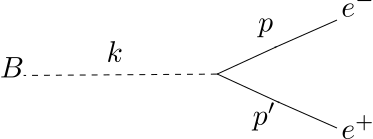
\includegraphics[scale=0.6]{Btoee} %noinstiki
  \caption{Feynman diagrams for $B\to e^+ e^-$} %noinstiki
  \label{fig:btoee} %noinstiki
\end{figure} %noinstiki
In the language of second quantization it is said that at the interaction point in Fig.~\ref{fig:btoee}, the scalar is destroyed by $\phi_+$ and one electron (${\psi_L}_-$) and a positron ($(\psi_R)^{\dagger}_{-}$) are created.

Let us define the one--particle states as in eq.~\eqref{eq:38f}

\begin{align}
  | H(\mathbf{p})\rangle\equiv\sqrt{\frac{1}{V}}a^\dagger_{\mathbf{p}}|0\rangle 
\end{align}
For the two Weyl spinors forming a Dirac spinor we have the solutions in eq.~\eqref{eq:fourweyl}, from here we can define the one--particle states were defined as in eq.~\eqref{eq:77f}
\begin{align}
   | e_L(\mathbf{p},s)\rangle\equiv&\sqrt{\frac{1}{V}}x_{\alpha}\left(s,\mathbf{p}\right) a^\dagger_s(\mathbf{p})|0\rangle, &    | e_R(\mathbf{p},s)\rangle\equiv&\sqrt{\frac{1}{V}}y^{\dagger\dot{\alpha}}\left(s,\mathbf{p}\right)a^\dagger_s(\mathbf{p})|0\rangle\nonumber\\
   | \left( e_L \right)^{\dagger}(\mathbf{p},s)\rangle\equiv&\sqrt{\frac{1}{V}}y_{\dot{\alpha}}^{\dagger}\left(s,\mathbf{p}\right){b}^\dagger_s(\mathbf{p})|0\rangle,&
   | \left( e_R \right)^{\dagger}(\mathbf{p},s)\rangle\equiv&\sqrt{\frac{1}{V}}x^{\alpha}\left(s,\mathbf{p}\right){b}^\dagger_s(\mathbf{p})|0\rangle\,.
\end{align}

Using the commutation relations, our states are then normalized as
\begin{align}
\langle H(\mathbf{p})| H(\mathbf{p}')\rangle=&\frac{(2\pi)^3}{V}\delta^3(\mathbf{p}-\mathbf{p}')\nonumber\\
\langle e_{L,R}(\mathbf{p},s)| e_{L,R}(\mathbf{p}',s')\rangle=&\frac{(2\pi)^3}{V}\delta_{s s'}\delta^3(\mathbf{p}-\mathbf{p}')\nonumber\\
\langle \left( e_{L,R} \right)^{\dagger}(\mathbf{p},s)| \left( e_{L,R} \right)^{\dagger}(\mathbf{p}',s')\rangle=&\frac{(2\pi)^3}{V}\delta_{s s'}\delta^3(\mathbf{p}-\mathbf{p}')
\end{align}
As established in Sec.~\ref{sec:fock-space-real}, it is convenient to work in the discrete limit where \eqref{eq:26f}
\begin{align}
   \delta^3(\mathbf{0})=\frac{V}{(2\pi)^3}\,.
\end{align}

Now we can write down the action of various field operators on different one particles states. 
Using the Fourier decomposition  of the scalar field in eq.~\eqref{eq:37f}, and taking into account that 
$a_{\mathbf{p}}|0\rangle=0$, we have
\begin{align}
\label{eq:98f}
   \phi_+(x)|H(\mathbf{k})\rangle=&\int d^3p \frac{1}{(2\pi)^3\sqrt{2\omega_{p} }}
\widehat{a}_{p} e^{-i p\cdot x }
|H(\mathbf{k})\rangle\nonumber\\
=&\int d^3p \frac{1}{(2\pi)^3\sqrt{2\omega_{p}}}
\widehat{a}_\mathbf{p} e^{-i p\cdot x }
\frac{1}{\sqrt{V}}\, \widehat{a}^\dagger_{\mathbf{k}}|0\rangle\nonumber\\
  =&\int d^3p \frac{1}{(2\pi)^3\sqrt{2\omega_{p}V}} e^{-i p\cdot x }
\, [\widehat{a}_{\mathbf{p}},\widehat{a}^\dagger_{\mathbf{k}}]|0\rangle\,.
\end{align}
%check normalization!
By using the commutation relations in eq.~\eqref{eq:32f} we have

\begin{align}
\phi_+(x)|H(\mathbf{k})\rangle  
=&\int d^3p \frac{\delta^{(3)}(\mathbf{p}-\mathbf{k})}{\sqrt{2\omega_{p}V}}
 e^{-i p\cdot x }|0\rangle
\end{align}
\begin{align}
\phi_+(x)|H(\mathbf{k})\rangle  
=&\frac{1}{\sqrt{2\omega_{k}V}}e^{-i k\cdot x }|0\rangle
\end{align}
Similarly, we have  \emph{initial one-particles states} on left and \emph{initial one-particles states} on right
\begin{align}
  \label{eq:99f}
  \phi_+(x)|H(\mathbf{k})\rangle=&\frac{1}{\sqrt{2 \omega_k V}}e^{-i k\cdot x}|0\rangle,&
 \langle H(\mathbf{k})|\phi_-(x)=&\langle0|\frac{1}{\sqrt{2 \omega_k V}}e^{i k\cdot x}\nonumber\\
  \xi_+(x)|e_{L}(\mathbf{p},s)\rangle=&\frac{1}{\sqrt{2 E_p V}}x(s,\mathbf{p})e^{-i p\cdot x}|0\rangle,&
  \langle e_{L}(\mathbf{p},s)|\xi_-^{\dagger}(x)=&\langle 0|\frac{1}{\sqrt{2 E_p V}}x^{\dagger}(s,\mathbf{p})e^{i p\cdot x}\nonumber\\
  \eta_+(x)|\left( e_R \right)^{\dagger}(\mathbf{p},s)\rangle=&\frac{1}{\sqrt{2 E_{p} V}}x(s,\mathbf{p})e^{-i p\cdot x}|0\rangle,&
  \langle \left( e_R \right)^{\dagger}(\mathbf{p},s)|\eta^{\dagger}_-(x)=&\langle 0|\frac{1}{\sqrt{2 E_{p} V}}x^{\dagger}(s,\mathbf{p})e^{i p\cdot x} \nonumber\\
  \xi_+^{\dagger}(x)|\left( e_{L} \right)^{\dagger}(\mathbf{p},s)\rangle=&\frac{1}{\sqrt{2 E_p V}}y^{\dagger}(s,\mathbf{p})e^{-i p\cdot x}|0\rangle,&
  \langle\left( e_{L} \right)^{\dagger}(\mathbf{p},s)|\xi_-(x)=&\langle 0| \frac{1}{\sqrt{2 E_p V}}y(s,\mathbf{p})e^{i p\cdot x}\nonumber\\
  \eta_+^{\dagger}(x)|e_R (\mathbf{p},s)\rangle=&\frac{1}{\sqrt{2 E_{p} V}}y^{\dagger}(s,\mathbf{p})e^{-i p\cdot x}|0\rangle,&
  \langle e_R(\mathbf{p},s)|\eta_-(x)=&\langle 0|\frac{1}{\sqrt{2 E_{p'} V}}y(s,\mathbf{p})e^{i p\cdot x}
 \,.
\end{align}
where $\omega_k$ and $E_p$ represent the energies of the scalar and the electron for the 3-momenta in the subscripts.

In the lowest order the only term which contributes to the matrix element is the term shown in Eq.~\eqref{eq:97f}.
The matrix element at first order in eq.~\eqref{eq:S1}, between the initial and the final state is then
\begin{align}
  S_{fi}^{(1)}=-i \frac{h}{\sqrt{2}} \sum_{s,s'} \int \operatorname{d}^4x &\left[ \left\langle 0, e_L(\boldsymbol{p}),\left( e_R \right)^{\dagger}(
\boldsymbol{p}') \left|\xi_-^{\dagger}(x)\eta_-^{\dagger}(x) \phi_{+}(x)  \right|H(\mathbf{k}),0,0 \right\rangle
   \right. +\nonumber\\
&\left.\left\langle 0,\left( e_L \right)^{\dagger}(\boldsymbol{p}), e_R (\boldsymbol{p}') \right|\xi_-(x)\eta_-(x) \phi_{+}(x)  \left|H(\mathbf{k}),0,0 \right\rangle \right] 
\end{align}
Using Eqs.~\eqref{eq:99f}  we obtain
\begin{align}
  S_{fi}^{(1)}=&(-i )\frac{h}{\sqrt{2}}  \sum_{s,s'}\left[ x^{\dagger}_{\dot{\alpha}}(s,\boldsymbol{p}){x^{\dagger}}^{\dot{\alpha}}(s',\boldsymbol{p}')+y^{\alpha}(s,\boldsymbol{p})y_{\alpha}(s',\boldsymbol{p}') \right] \nonumber\\
&\times\int d^4x\,e^{i(p+p'-k)\cdot x}\frac{1}{\sqrt{2\omega_k V}}\frac{1}{\sqrt{2E_p V}}\frac{1}{\sqrt{2E_{p'} V}}\,.
\end{align}
Since
\begin{align}
  \int d^4x\,e^{i(p+p'-k)\cdot x}=(2\pi)^4\delta^4(k-p-p')\,,
\end{align}
we obtain
\begin{align}
  S_{fi}^{(1)}=&\left[\frac{1}{\sqrt{2\omega_k V}}\frac{1}{\sqrt{2E_p V}}\frac{1}{\sqrt{2E_{p'} V}}\right]
(2\pi)^4\delta^4(k-p-p') \nonumber\\
&\times(-i )\frac{h}{\sqrt{2}}\sum_{s,s'}\left[ x^{\dagger}_{\dot{\alpha}}(s,\boldsymbol{p}){x^{\dagger}}^{\dot{\alpha}}(s',\boldsymbol{p}')+y^{\alpha}(s,\boldsymbol{p})y_{\alpha}(s',\boldsymbol{p}') \right].
\end{align}
Comparing with Eq.~\eqref{eq:RMfi} we have therefore that the relativistic \emph{amplitude} is
\begin{align}
\label{eq:calm}
  i\mathcal{M}_{fi}=-i \frac{h}{\sqrt{2}}\sum_{s,s'}\left[ x^{\dagger}_{\dot{\alpha}}(s,\boldsymbol{p}){x^{\dagger}}^{\dot{\alpha}}(s',\boldsymbol{p}')+y^{\beta}(s,\boldsymbol{p})y_{\beta}(s',\boldsymbol{p}') \right].
\end{align}
Check the specific calculation in~\ref{Dreiner:2008tw}

The equation for a two body decays, assuming that the amplitude \eqref{eq:calm} does not depends in the final momentum,  is given in eq.~\eqref{eq:152} is 
\begin{align}
\label{eq:154pdn}
\frac{d\Gamma}{d\Omega}=
&\frac{1}{64 \pi^2M^3}\left|\mathcal{M}_{fi}\right|^2\lambda^{1/2}(M^2,m_2^2,m_1^2)
\end{align}
where, from \eqref{eq:46}
\begin{align}
\label{eq:46n}
  \lambda(a,b,c)=\left[ a-(b-c) \right]^2-4ac\,.
\end{align}

For our specific problem, the final state masses of electron and positron is the same, however, we will obtain the results for the most general case of different masses. In this way, let $m$ ($m'=m$) the mass of $e_L$ ($e_R$).

The missing part is to calculate the square of the amplitude
\begin{align}
  \left| \mathcal{M} \right|^2=&\mathcal{M}^{\dagger}\mathcal{M}= \nonumber\\
=&\frac{h^{2}}{2}\sum_{s,s'}
 \left[ x^{\dagger}_{\dot{\alpha}}(s,\boldsymbol{p}){x^{\dagger}}^{\dot{\alpha}}(s',\boldsymbol{p}')+y^{\beta}(s,\boldsymbol{p})y_{\beta}(s',\boldsymbol{p}') \right]^{\dagger}
\left[ x^{\dagger}_{\dot{\alpha}}(s,\boldsymbol{p}){x^{\dagger}}^{\dot{\alpha}}(s',\boldsymbol{p}')+y^{\beta}(s,\boldsymbol{p})y_{\beta}(s',\boldsymbol{p}') \right] \nonumber\\
  =&\frac{h^2}{2}\sum_{s,s'} \left[x^{\alpha}(s',\boldsymbol{p}') x_{\alpha}(s,\boldsymbol{p})+y^{\dagger}_{\dot{\beta}}(s',\boldsymbol{p}')y^{\dagger\dot{\beta}}(s,\boldsymbol{p}) \right]
\left[ x^{\dagger}_{\dot{\alpha}}(s,\boldsymbol{p}){x^{\dagger}}^{\dot{\alpha}}(s',\boldsymbol{p}')+y^{\beta}(s,\boldsymbol{p})y_{\beta}(s',\boldsymbol{p}') \right],
\end{align}

 which includes (using anticommuting spinors)
\begin{align}
\sum_{s,s'}x^{\alpha}(s',\boldsymbol{p}') x_{\alpha}(s,\boldsymbol{p})
x^{\dagger}_{\dot{\alpha}}(s,\boldsymbol{p}){x^{\dagger}}^{\dot{\alpha}}(s',\boldsymbol{p}') 
&= \sum_{s'}x^{\alpha}(s',\boldsymbol{p}')  \left[ 
\sum_{s} x_{\alpha}(s,\boldsymbol{p})x^{\dagger}_{\dot{\alpha}}(s,\boldsymbol{p})\right]
{x^{\dagger}}^{\dot{\alpha}}(s',\boldsymbol{p}')  \nonumber\\
&= \sum_{s'}x^{\alpha}(s',\boldsymbol{p}') \left( p\cdot \sigma_{\alpha{\dot{\alpha}}}  \right)
{x^{\dagger}}^{\dot{\alpha}}(s',\boldsymbol{p}')  \nonumber\\
&=\left( p\cdot \sigma_{\alpha{\dot{\alpha}}}  \right) \sum_{s'} {x^{\dagger}}^{\dot{\alpha}}(s',\boldsymbol{p}') x^{\alpha}(s',\boldsymbol{p}')  \nonumber\\
&=\left( p\cdot \sigma_{\alpha{\dot{\alpha}}}  \right) \left( p'\cdot \overline{\sigma}^{\dot{\alpha}\alpha} \right) \nonumber\\
&=\operatorname{Tr}\left[ \left( p\cdot \sigma \right)\left( p'\cdot \overline{\sigma} \right)  \right] \nonumber\\
&=p_{\mu}p'_{\nu}\operatorname{Tr}\left[ \sigma^{\mu} \overline{\sigma}^{\nu}  \right] \nonumber\\ 
&=2 g^{\mu\nu}p_{\mu}p'_{\nu} \nonumber\\
&=2 p\cdot p'\,.
\end{align}

\begin{align}
\sum_{s,s'}y^{\dagger}_{\dot{\beta}}(s',\boldsymbol{p}')y^{\dagger\dot{\beta}}(s,\boldsymbol{p})y^{\beta}(s,\boldsymbol{p})y_{\beta}(s',\boldsymbol{p}')
=&  \left( p\cdot \overline{\sigma}^{\dot{\beta}\beta} \right)\sum_{s,s'}y^{\dagger}_{\dot{\beta}}(s',\boldsymbol{p}')y_{\beta}(s',\boldsymbol{p}') \nonumber\\
=&  \left( p\cdot \overline{\sigma}^{\dot{\beta}\beta} \right) \sum_{s,s'}y_{\beta}(s',\boldsymbol{p}')y^{\dagger}_{\dot{\beta}}(s',\boldsymbol{p}') \nonumber\\
=&  \left( p\cdot \overline{\sigma}^{\dot{\beta}\beta} \right) \left( p'\cdot \sigma_{\beta \dot{\beta}} \right) \nonumber\\
=& 2 p \cdot p'\,.
\end{align}

\begin{align}
  \sum_{s,s'}x^{\alpha}(s',\boldsymbol{p}') x_{\alpha}(s,\boldsymbol{p})y^{\beta}(s,\boldsymbol{p})y_{\beta}(s',\boldsymbol{p}') =& 
  \sum_{s'}x^{\alpha}(s',\boldsymbol{p}') \left[ \sum_{s} x_{\alpha}(s,\boldsymbol{p})y^{\beta}(s,\boldsymbol{p}) \right]y_{\beta}(s',\boldsymbol{p}') \nonumber\\
 =& \left(m{\delta_{\alpha}}^{\beta}  \right) \sum_{s'}  y_{\beta}(s',\boldsymbol{p}')x^{\alpha}(s',\boldsymbol{p}') \nonumber\\
 =& \left(m{\delta_{\alpha}}^{\beta}  \right)  \left(- m'{{\delta_{\beta}}^{\alpha}}  \right) \nonumber\\
 =& \operatorname{Tr} \left[ -m m'  \boldsymbol{1} \boldsymbol{1} \right] \nonumber\\
 =& mm'\operatorname{Tr} \left[  \boldsymbol{1} \right] \nonumber\\
 =& -2 mm'\,.
\end{align}

\begin{align}
  \sum_{s,s'}y^{\dagger}_{\dot{\beta}}(s',\boldsymbol{p}')y^{\dagger\dot{\beta}}(s,\boldsymbol{p})x^{\dagger}_{\dot{\alpha}}(s,\boldsymbol{p}){x^{\dagger}}^{\dot{\alpha}}(s',\boldsymbol{p}')  
=&   \left( m {\delta^{\dot{\beta}}}_{\dot{\alpha}} \right) \left( -m' {\delta}^{\dot{\alpha}}_{\dot{\beta}} \right) \nonumber\\
=& -2m m'\,.
\end{align}
Therefore
\begin{align}
   \left| \mathcal{M} \right|^2=4 \frac{h^{2}}{2} \left( p\cdot p' - mm' \right)
\end{align}

From the conservation of the momentum-energy in the center of mass frame
\begin{align}
  k^{\mu}=&\left(M,\boldsymbol{0}\right) \nonumber\\
  p^{\mu}=&\left(E,\boldsymbol{p}\right) \nonumber\\
  {p'}^{\mu}=&\left(E',\boldsymbol{p}'\right) \,,
\end{align}
as assummed in \eqref{eq:154pdn}, we have
\begin{align}
  k^{\mu}=p^{\mu}+{p'}^{\mu},,
\end{align}
which implies for each component that
\begin{align}
  M=&E+{E'}\nonumber\\
|\mathbf{p}|&=|\mathbf{p}'|.
\end{align}
From the first equation
\begin{align}
  M^2=E^2+{E'}^2+2EE'\,.
\end{align}
Therefore
\begin{align}
  E{E'}=\frac{M^2-E^2-{E'}^2}{2}
\end{align}
\begin{align*}
  p\cdot p'-m {m'}&=EE'-\mathbf{p}\cdot\mathbf{p}'-m {m'}\\
&=EE'+\mathbf{p}^2-m {m'}\\
&=\frac{M^2-E^2-{E'}^2}{2}+\mathbf{p}^2-m {m'}\nonumber\\
&=\frac12\left(M^2-m^2-\mathbf{p}^2-{m'}^2-\mathbf{p}^2\right)+\mathbf{p}^2-m {m'}\\
&=\frac12\left(M^2-m^2-{m'}^2-2m{m'}\right)\\
&=\frac12\left[M^2-(m-{m'})^2\right]
\end{align*}
%\left(\right)
Therefore, the scattering  amplitude is
\begin{equation}
\sum_{s_1,s_2}|\mathcal{M}|^{2}=h^2\left[M^2-(m+{m'})^2\right]
\end{equation}
Since this does not depends explicitly on the final state tri-momentum, is was consistent to already make the tri-momentum integrals. Moreower, Replacing back in eq.~\eqref{eq:154pdn}
\begin{align}
\frac{d\Gamma}{d\Omega}=
&\frac{h^2}{64 \pi^2M^3}\lambda^{1/2}(M^2,{m'}^2,m^2)\left[M^2-(m+{m'})^2\right]
\end{align}
After the integration $\int d\Omega_{\text{CM}}=4\pi$\footnote{$\int_0^{2\pi}d\phi\int_0^\pi\sin\theta d\theta=4\pi $} we have
\begin{align}
\Gamma=&\frac{h^2}{16 \pi M^3}\lambda^{1/2}(M^2,{m'}^2,m^2)\left[M^2-(m+{m'})^2\right]
\end{align}
For $m={m'}=m_f$, and using eq.~\eqref{eq:46n}


\begin{align}
  \lambda^{1/2}(M^2,m^2_f,m_f^2)=&
  \left[ \left( M^2-m^2_f+m^2_f  \right)^2-4 M^2m_f^2  \right]^{1/2}\nonumber\\
  =&\left( M^4-4 M^2m_f^2  \right)^{1/2}\nonumber\\
  =&\left[M^4 \left( 1-4 \frac{m_f^2}{M^2} \right) \right]^{1/2}\nonumber\\
  =&M^2 \left( 1-4 \frac{m_f^2}{M^2} \right)^{1/2}\,,
\end{align}
and therefore
\begin{align}
\Gamma(H\to f\overline{f})=&\frac{h^2}{16 \pi M^3}M^2 \left( 1-4 \frac{m_f^2}{M^2} \right)^{1/2}
 \left[M^2-4m_f^2\right] \nonumber\\
=&\frac{h^2}{16 \pi M^3}M^4 \left( 1-4 \frac{m_f^2}{M^2} \right)^{1/2}
 \left[1-4 \frac{m_f^2}{M^2}\right] \nonumber\\
=&\frac{h^2}{16 \pi}M\left(1-\frac{4m_f^2}{M^2}\right)^{3/2}
\end{align}
In the case of the standard model Higgs with mass $M_H=M$ decaying to fermion pair, and using $m_f=hv/\sqrt{2}$,  $v=\left( \sqrt{2}G_F \right)^{-1/2}$

\begin{align}
\Gamma(H\to f\overline{f})=&\frac{h^2v^2}{16 v^2 \pi}M_H\left(1-\frac{4m_f^2}{M_H^2}\right)^{3/2} \nonumber\\
=&\frac{h^2v^2}{2}\frac{1}{8 v^2 \pi}M_H\left(1-\frac{4m_f^2}{M_H^2}\right)^{3/2} \nonumber\\
=&m_f^2\frac{\sqrt{2}G_F}{8\pi}M_H\left(1-\frac{4m_f^2}{M_H^2}\right)^{3/2} \nonumber\\
&=\frac{M_{H}m_{f}^{2}G_{F}}{4\pi\sqrt{2}}
\left(1-4\frac{m^2_{f}}{M^2_{H}}\right)^{3/2}, 
\end{align}

In the limit $m_{f}\ll M_{H}$ this expression reduces to 
\begin{equation}
\Gamma(H\to
f\overline{f})=\frac{M_{H}m_{f}^{2}G_{F}}{4\pi\sqrt{2}}. 
\end{equation}
For the tau\footnote{to the top quarks is kinematically forbidden, to the bottom quark a further factor $N_c=3$ must be considered}, taking into account that $1.166 \times 10^{-5}\ \text{GeV}^{-2}$, $M_H=125\ \text{GeV}$, and $m_\tau=1.777\ \text{GeV}$,
\begin{align}
  \Gamma(H\to \tau^+\tau^-)=0.26\ \text{MeV}\to \tau= \frac{\hbar}{\Gamma}=2.53\times 10^{-21}\ \text{seconds}\,.
\end{align}
\end{frame}



% \subsection{Yukawa interaction for Weyl fermions}
% Left-handed fermion:
% \begin{align}
% %e_L -> e_L^- + (e_R^+)^{\dagger}
% e_L\to  \xi_{\alpha}=&\int \frac{d^3 p}{(2\pi)^3\sqrt{2E_{\mathbf{p}}}} \left[ x_{\alpha}(\mathbf{p},s)a(\mathbf{p},s)\operatorname{e}^{-i p\cdot x}+y_{\alpha}(\mathbf{p},s)a^{\dagger}(\mathbf{p},s)\operatorname{e}^{i p\cdot x} \right] \nonumber\\
% %(e_L)^{\dagger} -> e_R^+ + (e_L^-)^{\dagger}
% \left( e_L \right)^{\dagger}\to  \xi_{\dot{\alpha}}^{\dagger}=&\int \frac{d^3 p}{(2\pi)^3\sqrt{2E_{\mathbf{p}}}} \left[y_{\dot{\alpha}}^{\dagger}(\mathbf{p},s)a(\mathbf{p},s)\operatorname{e}^{-i p\cdot x}+ x_{\dot{\alpha}}^{\dagger}(\mathbf{p},s)a^{\dagger}(\mathbf{p},s)\operatorname{e}^{i p\cdot x}\right] .
% \end{align}

% Right-handed fermion 
% \begin{align}
% %e_R -> e_R^- + (e_L^+)^{\dagger}
% e_R\to  \eta^{\dagger\dot{\alpha}}=&\int \frac{d^3 p}{(2\pi)^3\sqrt{2E_{\mathbf{p}}}} \left[y^{\prime\dot{\alpha}\dagger}(\mathbf{p},s)b(\mathbf{p},s)\operatorname{e}^{-i p\cdot x}+ x^{\prime\dot{\alpha}\dagger}(\mathbf{p},s)b^{\dagger}(\mathbf{p},s)\operatorname{e}^{i p\cdot x} \right] .
%  \nonumber\\
% %(e_R)^{\dagger} -> e_L^+ + (e_R^-)^{\dagger}
% \left( e_R \right)^{\dagger}\to  \eta^{\alpha}=&\int \frac{d^3 p}{(2\pi)^3\sqrt{2E_{\mathbf{p}}}} \left[ x^{\prime\alpha}(\mathbf{p},s)b(\mathbf{p},s)\operatorname{e}^{-i p\cdot x}+y^{\prime\,\alpha}(\mathbf{p},s)b^{\dagger}(\mathbf{p},s)\operatorname{e}^{i p\cdot x} \right]
% \end{align}
% \begin{align}
%  \xi_{+} | e^{-}_{L}\rangle =& x a a^{\dagger} |0\rangle \nonumber\\
%  \eta_{+} | \left( e^{-}_{R} \right)^{\dagger}\rangle =& x' b b^{\dagger} |0\rangle \nonumber\\
%  \xi_{+} |  \left( e^{-}_{L} \right)^{\dagger} \rangle =& y^{\dagger} a a^{\dagger} |0\rangle \nonumber\\
%  \eta_{+} | e^{-}_{R} \rangle =& y^{\prime \dagger} b b^{\dagger} |0\rangle
% \end{align}
% After some calcultations ...

% From the cojugate relations, e.g $\langle e_L^- |\xi_-=\langle 0|x^{\dagger}...$, etc
% \begin{align}
%   \mathcal{M}_1 =& x^{\dagger} x^{\prime \dagger} &\mathcal{M}_2=& y y'
% \end{align}
\section{Wick Theorem}
\label{sec:wick-theorem}

\subsection{Basics concepts}
Return back to  the interpretation of interaction in terms of one exchanged particle, as illustrated again in Fig.~\ref{fig:qedrepulsionx1x2}
\begin{figure}
  \centering
  \includegraphics{qedrepulsionx1x2}
  \caption{Electromagnetic repulsion. The diagrams (a) and (b) are summarized in the diagram (c)}
  \label{fig:qedrepulsionx1x2}
\end{figure}


From \cite{Lahiri:2005sm}. The normal ordering procedure involved putting all the annihilation operators to the right of all creation operators so that it annihilates the vacuum. But the time ordering raises complications because in it all operators at earlier times must be further to the right. So creation operators at later times would be to the right of annihilation operators at later times, contrary to what we need for normal ordering. The advantage of normal ordered products is that their expectation values vanish in the vacuum. 

If $H_{\text{int}}$ contains an even number of fermion factors, we can use the time--ordered product $\operatorname{T}\{\ldots\}$ of $n$ factors to write this expression in the equivalent form. For $S^{(2)}$ we have for example
\begin{align}
 \int_{-\infty}^\infty \operatorname{d}t_1 \int_{-\infty}^{\infty}\operatorname{d}t_2 \operatorname{T}\{H_{\text{int}}(t_1)H_{\text{int}}(t_2)\}=&
\int_{-\infty}^\infty \operatorname{d}t_1\int_{-\infty}^{\infty}\operatorname{d}t_2 \theta(t_2-t_1)H_{\text{int}}(t_2)H_{\text{int}}(t_1) \nonumber\\
&+\int_{-\infty}^\infty \operatorname{d}t_1\int_{-\infty}^{\infty}\operatorname{d}t_2 \theta(t_1-t_2)H_{\text{int}}(t_1)H_{\text{int}}(t_2)
 \end{align}
where, for $t_2$ and $t_1$ fixed respectively
 \begin{align}
   \theta(t_2-t_1)=&
   \begin{cases}
    0\, &    t_1> t_2\\
    1\, &    t_1< t_2\\
   \end{cases},&   \theta(t_1-t_2)=&
   \begin{cases}
    0\, &    t_2> t_1\\
    1\, &    t_2< t_1\\
   \end{cases}\,.
 \end{align}
In this way.
\begin{align}
 \int_{-\infty}^\infty \operatorname{d}t_1 \int_{-\infty}^{\infty}\operatorname{d}t_2 \operatorname{T}\{H_{\text{int}}(t_1)H_{\text{int}}(t_2)\}=&
\int_{-\infty}^\infty \operatorname{d}t_2\int_{-\infty}^{t_2}\operatorname{d}t_1 \theta(t_2-t_1)H_{\text{int}}(t_2)H_{\text{int}}(t_1)\nonumber\\
&+\cancel{\int_{-\infty}^\infty \operatorname{d}t_2\int_{t_2}^{t_1}\operatorname{d}t_1 \theta(t_2-t_1)H_{\text{int}}(t_2)H_{\text{int}}(t_1)} \nonumber\\
&+\int_{-\infty}^\infty \operatorname{d}t_1\int_{-\infty}^{t_{1}}\operatorname{d}t_2 \theta(t_1-t_2)H_{\text{int}}(t_1)H_{\text{int}}(t_2) \nonumber\\
&+\cancel{\int_{-\infty}^\infty \operatorname{d}t_1\int_{t_1}^{t_2}\operatorname{d}t_2 \theta(t_1-t_2)H_{\text{int}}(t_1)H_{\text{int}}(t_2)}\,.
\end{align}
The integral in $\operatorname{d}t_1$ is for $t_1>t_2$, with $t_2$ fixed, so that $\theta(t_2-t_1)=0$ for $t_1>t_2$. Similarly,
The integral in $\operatorname{d}t_2$ is for $t_2>t_1$, with $t_1$ fixed, so that $\theta(t_1-t_2)=0$ for $t_2>t_1$. Therefore,
\begin{align}
   \int_{-\infty}^\infty \operatorname{d}t_1 \int_{-\infty}^{\infty}\operatorname{d}t_2 \operatorname{T}\{H_{\text{int}}(t_1)H_{\text{int}}(t_2)\}=&
\int_{-\infty}^\infty \operatorname{d}t_2\int_{-\infty}^{t_2}\operatorname{d}t_1 H_{\text{int}}(t_2)H_{\text{int}}(t_1)
+\int_{-\infty}^\infty \operatorname{d}t_1\int_{-\infty}^{t_{1}}\operatorname{d}t_2 H_{\text{int}}(t_1)H_{\text{int}}(t_2)\nonumber\\
=&
\int_{-\infty}^\infty \operatorname{d}t_1\int_{-\infty}^{t_1}\operatorname{d}t_2 H_{\text{int}}(t_1)H_{\text{int}}(t_2)
+\int_{-\infty}^\infty \operatorname{d}t_1\int_{-\infty}^{t_{1}}\operatorname{d}t_2 H_{\text{int}}(t_1)H_{\text{int}}(t_2) \nonumber\\
=&
2\int_{-\infty}^\infty \operatorname{d}t_1\int_{-\infty}^{t_1}\operatorname{d}t_2 H_{\text{int}}(t_1)H_{\text{int}}(t_2)\,.
\end{align}
In terms of the ordering operator all the integrals are between $-\infty$ to $\infty$:
\begin{align}
   S=&1+\sum_{n=1}^\infty\frac{(-i)^n}{n!}\int_{-\infty}^{\infty}\operatorname{d}t_1\,\int_{-\infty}^{\infty} \operatorname{d}t_2\ldots\int_{-\infty}^{\infty}\operatorname{d}t_n\,\operatorname{T}\{{H}_{\text{int}}(t_1){H}_{\text{int}}(t_2)\ldots{H}_{\text{int}}(t_n)\}\,, 
\end{align}
In terms of the Hamiltonian density, we have
\begin{align}
  S=1+\sum_{n=1}^\infty\frac{(-i)^n}{n!}\int\cdots\int d^4x_1 d^4x_2\ldots d^4x_n\,\operatorname{T}\{\mathcal{H}_{\text{int}}(x_1)\mathcal{H}_{\text{int}}(x_2)\ldots\mathcal{H}_{\text{int}}(x_n)\}\,, 
\end{align}
In the above perturbation formalism the states $|i\rangle$ and $|f\rangle$ are, as usual, eigenstates of the unperturbed free-field Hamiltonian $H_0$. As such can be introduced inside the integrals
\begin{align}
  S_{f i}=&\langle f|S|i\rangle\nonumber\\
  =&1+\sum_{n=1}^\infty\frac{(-i)^n}{n!}\int\cdots\int d^4x_1 d^4x_2\ldots d^4x_n\,\langle f|\operatorname{T}\{\mathcal{H}_{\text{int}}(x_1)\mathcal{H}_{\text{int}}(x_2)\ldots\mathcal{H}_{\text{int}}(x_n)\}|i\rangle\,.
\end{align}


For example, at first order
\begin{align}
  \label{eq:96f}
  S_{fi}^{(1)}=&\langle f|S^{(1)}|i\rangle\nonumber\\
  =&\langle f|-i\int d^4x_1\,\operatorname{T}\{\mathcal{H}_{\text{int}}(x_1)\}|i\rangle\nonumber\\
  =&-i\int d^4x_1\,\langle f|:\mathcal{H}_{\text{int}}(x_1):|i\rangle\,.
\end{align}
In order to evaluate this integrals we need to write the time ordered product in terms of the fields. This can done by induction. We start by considering the simple no trivial case with two scalar fields
%ver cuaderno de perrito



\subsection{Wick theorem}
To evaluate the time-ordered product we need first to show that
\begin{align}
 \operatorname{T}\{\phi(x_1)\phi(x_2)\}=:\phi(x_1)\phi(x_2):+\langle0|\operatorname{T}\{\phi(x_1)\phi(x_2)\}|0\rangle\,,
\end{align}
where the last term
\begin{align}
  i\Delta_F(x_1-x_2)=&\langle0|\operatorname{T}\{\phi(x_1)\phi(x_2)\}|0\rangle\,
\end{align}
corresponds to the \emph{scalar propagator}. The demostration is displayed below.

%copy and paste from scanned pages below
We can rewrite the scalar propagator in terms of 
the Wick contraction, which is defined just as:
\begin{align}
\label{eq:77f}
  \bcontraction{\,}{\phi}{(x_1)}{\phi}
\,\phi(x_1)\phi(x_2)=&\langle0|\operatorname{T}\{\phi(x_1)\phi(x_2)\}|0\rangle\,.
\end{align}

We can then stablish the Wick theorem as
\begin{align}
 \operatorname{T}\{\phi(x_1)\phi(x_2)\}=:\phi(x_1)\phi(x_2):+\bcontraction{\,}{\phi}{(x_1)}{\phi}
\,\phi(x_1)\phi(x_2)\,.
\end{align}
For the demostration


since
\begin{align}
  \phi(x)=\phi_+(x)+\phi_-(x)\,,
\end{align}
\begin{align}
\operatorname{T}\left[\phi(x_1),\phi(x_2)\right]=\theta(t_1-t_2)\phi(x_1)\phi(x_2)+\theta(t_2-t_1)\phi(x_2)\phi(x_1)
\end{align}
\begin{align}
    \langle0|\operatorname{T}\left[\phi(x_1),\phi(x_2)\right]|0\rangle=&\theta(t_1-t_2)\langle0|\phi(x_1)\phi(x_2)|0\rangle+\theta(t_2-t_1)\langle0|\phi(x_2)\phi(x_1)|0\rangle\nonumber\\
   =&\theta(t_1-t_2)\langle0|\phi_+(x_1)\phi_-(x_2)|0\rangle+\theta(t_2-t_1)\langle0|\phi_+(x_2)\phi_-(x_1)|0\rangle\nonumber\\
     =&\langle0|\theta(t_1-t_2)\phi(x_1)_+\phi_-(x_2)|0\rangle+\langle0|\theta(t_2-t_1)\phi_+(x_2)\phi_-(x_1)|0\rangle
\end{align}

with
\begin{align}
    \phi_+(x)=&\int \operatorname{d}^3p \frac{1}{(2\pi)^3\sqrt{2\omega_{\boldsymbol{p}} }}
\widehat{a}_{\boldsymbol{p}} e^{-i p\cdot x }&
    \phi_-(x)=&\int \operatorname{d}^3p \frac{1}{(2\pi)^3\sqrt{2\omega_{\boldsymbol{p}} }}
\widehat{a}_{\boldsymbol{p}}^\dagger e^{i p\cdot x }\,,
\end{align}
we have
\begin{align}
  \langle0|T(\phi(x_1)\phi(x_2))|0\rangle
=&\langle0|\int\frac{\operatorname{d}^3p_1}{(2\pi)^3\sqrt{2E_{\boldsymbol{p}_1}}}\theta(t_1-t_2)\hat{a}_{\boldsymbol{p}_1}e^{-i p_1\cdot x_1}
\int\frac{\operatorname{d}^3p_2}{(2\pi)^3\sqrt{2E_{\boldsymbol{p}_2}}}\hat{a}_{\boldsymbol{p}_2}^\dagger e^{-i p_2\cdot x_2}|0\rangle\nonumber\\
&+\langle0|\int\frac{\operatorname{d}^3p_2}{(2\pi)^3\sqrt{2E_{\boldsymbol{p}_2}}}\theta(t_2-t_1)\hat{a}_{\boldsymbol{p}_2}e^{-i p_2\cdot x_2}
\int\frac{\operatorname{d}^3p_1}{(2\pi)^3\sqrt{2E_{\boldsymbol{p}_1}}}\hat{a}_{\boldsymbol{p}_1}^\dagger e^{-i p_1\cdot x_1}|0\rangle\nonumber\\
=&\int\int\frac{\operatorname{d}^3p_1\operatorname{d}^3p_2}{(2\pi)^6\sqrt{2E_{\boldsymbol{p}_1}}\sqrt{2E_{\boldsymbol{p}_2}}}\theta(t_1-t_2)e^{-i p_1\cdot x_1}e^{-i p_2\cdot x_2}
\langle0|\hat{a}_{\boldsymbol{p}_1}\hat{a}_{\boldsymbol{p}_2}^\dagger|0\rangle\nonumber\\
&+\int\int\frac{\operatorname{d}^3p_2\operatorname{d}^3p_1}{(2\pi)^6\sqrt{2E_{\boldsymbol{p}_2}}\sqrt{2E_{\boldsymbol{p}_1}}}\theta(t_2-t_1)e^{-i p_2\cdot x_2}e^{-i p_1\cdot x_1}
\langle0|\hat{a}_{\boldsymbol{p}_2}\hat{a}_{\boldsymbol{p}_1}^\dagger|0\rangle\,,
\end{align}
In this way
\begin{align}
 \langle0|T(\phi(x_1)\phi(x_2))|0\rangle
  =\int\int\frac{\operatorname{d}^3p_1\operatorname{d}^3p_2}{(2\pi)^6\sqrt{2E_{\boldsymbol{p}_1}2E_{\boldsymbol{p}_2}}}
&\left[\theta(t_1-t_2)e^{-i p_1\cdot x_1}e^{-i p_2\cdot x_2}
\langle0|\hat{a}_{\boldsymbol{p}_1}\hat{a}_{\boldsymbol{p}_2}^\dagger|0\rangle \right. \nonumber\\
&\left.  + \theta(t_2-t_1)e^{-i p_2\cdot x_2}e^{-i p_1\cdot x_1}
\langle0|\hat{a}_{\boldsymbol{p}_2}\hat{a}_{\boldsymbol{p}_1}^\dagger|0\rangle \right]
\end{align}



and the final result is that
\begin{align}
  \langle0|T(\phi(x_1)\phi(x_2))|0\rangle=\int \frac{\operatorname{d}^{4} p}{(2 \pi)^{4}} \frac{e^{-i p \cdot\left(x_1-x_2\right)}}{p^2-m^2-i \varepsilon}
\end{align}

\includepdf[pages=-]{propagator.pdf}  

\includepdf[pages=-]{wick.pdf}  


 Generalizing  the results for $n$ scalar or fermion fields, but with an even number of fermions fields, we have the Wick theorem
\begin{align}
  \operatorname{T}\{\Phi(x_1)\Phi(x_2)\Phi(x_3)\cdots\Phi(x_n) \}
=&:\Phi(x_1)\Phi(x_2)\Phi(x_3)\cdots\Phi(x_n):+\nonumber\\
&+\bcontraction{\,}{\Phi}{(x_1)}{\Phi}\,\Phi(x_1)\Phi(x_2):\Phi(x_3)\cdots\Phi(x_n):\nonumber\\
&+:\Phi(x_1)\bcontraction{\,}{\Phi}{(x_2)}{\Phi}\,\Phi(x_2)\Phi(x_3)\cdots\Phi(x_n):+\cdots  \nonumber\\
=&:\Phi(x_1)\Phi(x_2)\Phi(x_3)\cdots\Phi(x_n):+\nonumber\\
&+\left[:\bcontraction{\,}{\Phi}{(x_1)}{\Phi}\,\Phi(x_1)\Phi(x_2)\Phi(x_3)\cdots\Phi(x_n): +\text{perm} \right]\nonumber\\
&+\left[  :\bcontraction{\,}{\Phi}{(x_1)}{\Phi}\,\Phi(x_1)\Phi(x_2) \bcontraction{\,}{\Phi}{(x_3)}{\Phi}\,\Phi(x_3)\Phi(x_4)\Phi(x_5)\cdots\Phi(x_n): +\text{perm}  \right] \nonumber\\
&+\cdots \nonumber\\
\end{align}
For details of the full result see for example \cite{Lahiri:2005sm}.


\section{Mandelstam variables}

We can generalize the definition of $s$ in eq.\eqref{eq:smv} to the full
Mandelstam variables \url{http://bolvan.ph.utexas.edu/~vadim/Classes/2011f/STU.pdf}, (See also \cite{Peskin})
\begin{align}
\label{eq:mvstu}
  s=&\left( p_1+p_2 \right)^2=\left( p_1'+p_2' \right)^2 \nonumber\\
  t=&\left( p_1-p_1' \right)^2=\left( p_2-p_2' \right)^2 \nonumber\\
  u=&\left( p_1-p_2' \right)^2=\left( p_1'-p_2 \right)^2 \,.
\end{align}
The explicit form for $s$ is 
\begin{align}
  s=&\left( p_1+p_2 \right)^2 \nonumber\\
 =& p_1^2+p_2^2+2 p_1\cdot p_2 \nonumber\\
=& m_1^2+m_2^2+2 p_1\cdot p_2\,,
\end{align}
from which the product $p_1\cdot p_2$ can be obtained.  By following similar steps for $t$ and $u$, we have
\begin{align}
\label{eq:stucs}
  2 p_1\cdot p_2=&s- m_1^2-m_2^2 \nonumber\\
  2 p_1'\cdot p_2'=&s- {m_1'}^2-{m_2'}^2 \nonumber\\
  2 p_1\cdot p_1'=&m_1^2+{m_1'}^2 -t \nonumber\\
  2 p_2\cdot p_2'=&m_2^2+{m_2'}^2 -t \nonumber\\
  2 p_1\cdot p_2'=&m_1^2+{m_2'}^2 -u \nonumber\\
  2 p_2\cdot p_1'=&m_2^2+{m_1'}^2 -u \,.
\end{align}
Moreover,
\begin{align}
  s+t+u=m_1^2+m_2^2+{m_1'}^2+{m_2'}^2\,.
\end{align}

In the non-relativistic limit
\begin{align}
  s&=m_1^2+m_2^2   +2 p_1\cdot p_2 \approx (m_1+m_2)^2  + m_1m_2 (\mathbf{v}_1-\mathbf{v}_2)>0\,, \nonumber\\
  t&=m_1^2+{m_1'}^2-2 p_1\cdot p_1'\approx (m_1-m_1')^2 - m_1m_1' (\mathbf{v}_1-\mathbf{v}_1')>0\,,\nonumber\\
  u&=m_1^2+{m_2'}^2-2 p_1\cdot p_2'\approx (m_1-m_2')^2 - m_1m_2'  (\mathbf{v}_1-\mathbf{v}_2')>0\,.
\end{align}
In the center of mass frame ($\boldsymbol{p}_1+\boldsymbol{p}_1=0$)
\begin{align}
  s=\left( E_1+\boldsymbol{p}_1+E_2+\boldsymbol{p}_2 \right)^2=\left( E_1+\boldsymbol{p}_1+E_2-\boldsymbol{p}_1 \right)^2=\left( E_1+E_2 \right)^2.
\end{align} 


%%% Local Variables: 
%%% mode: latex
%%% TeX-master: "beyond"
%%% End: